

For the last test case the method without additional gradient jump lacks convergence as in the previous test cases. We therefore concentrate on the variant penalising the gradient normal jump across edges. The plots of the error can be found in Figure \ref{fig: l2 errors test 4 jump} and Figure \ref{fig: h1 errors test 4 jump}, as well as in Table \ref{tab: l2 errors test 4 jump}. Again Newton's method did not converge on fine grids for $k=2$ or $k=3$.

As before we do not observe much difference between the choices $k=2$ and $k=3$ during the first refinements where the method still converges. But as the Aleksandrov solution of this test case lacks regularity it is not surprising that increasing the polynomial degree does not effect the error.

It is noticeable that for $k=2$ the $L^2$ error increases after four refinements while the $H^1$ error decreases. We already experienced this behaviour in test \ref{test smooth}.

\begin{figure}[h]
	\centering
		\centering
		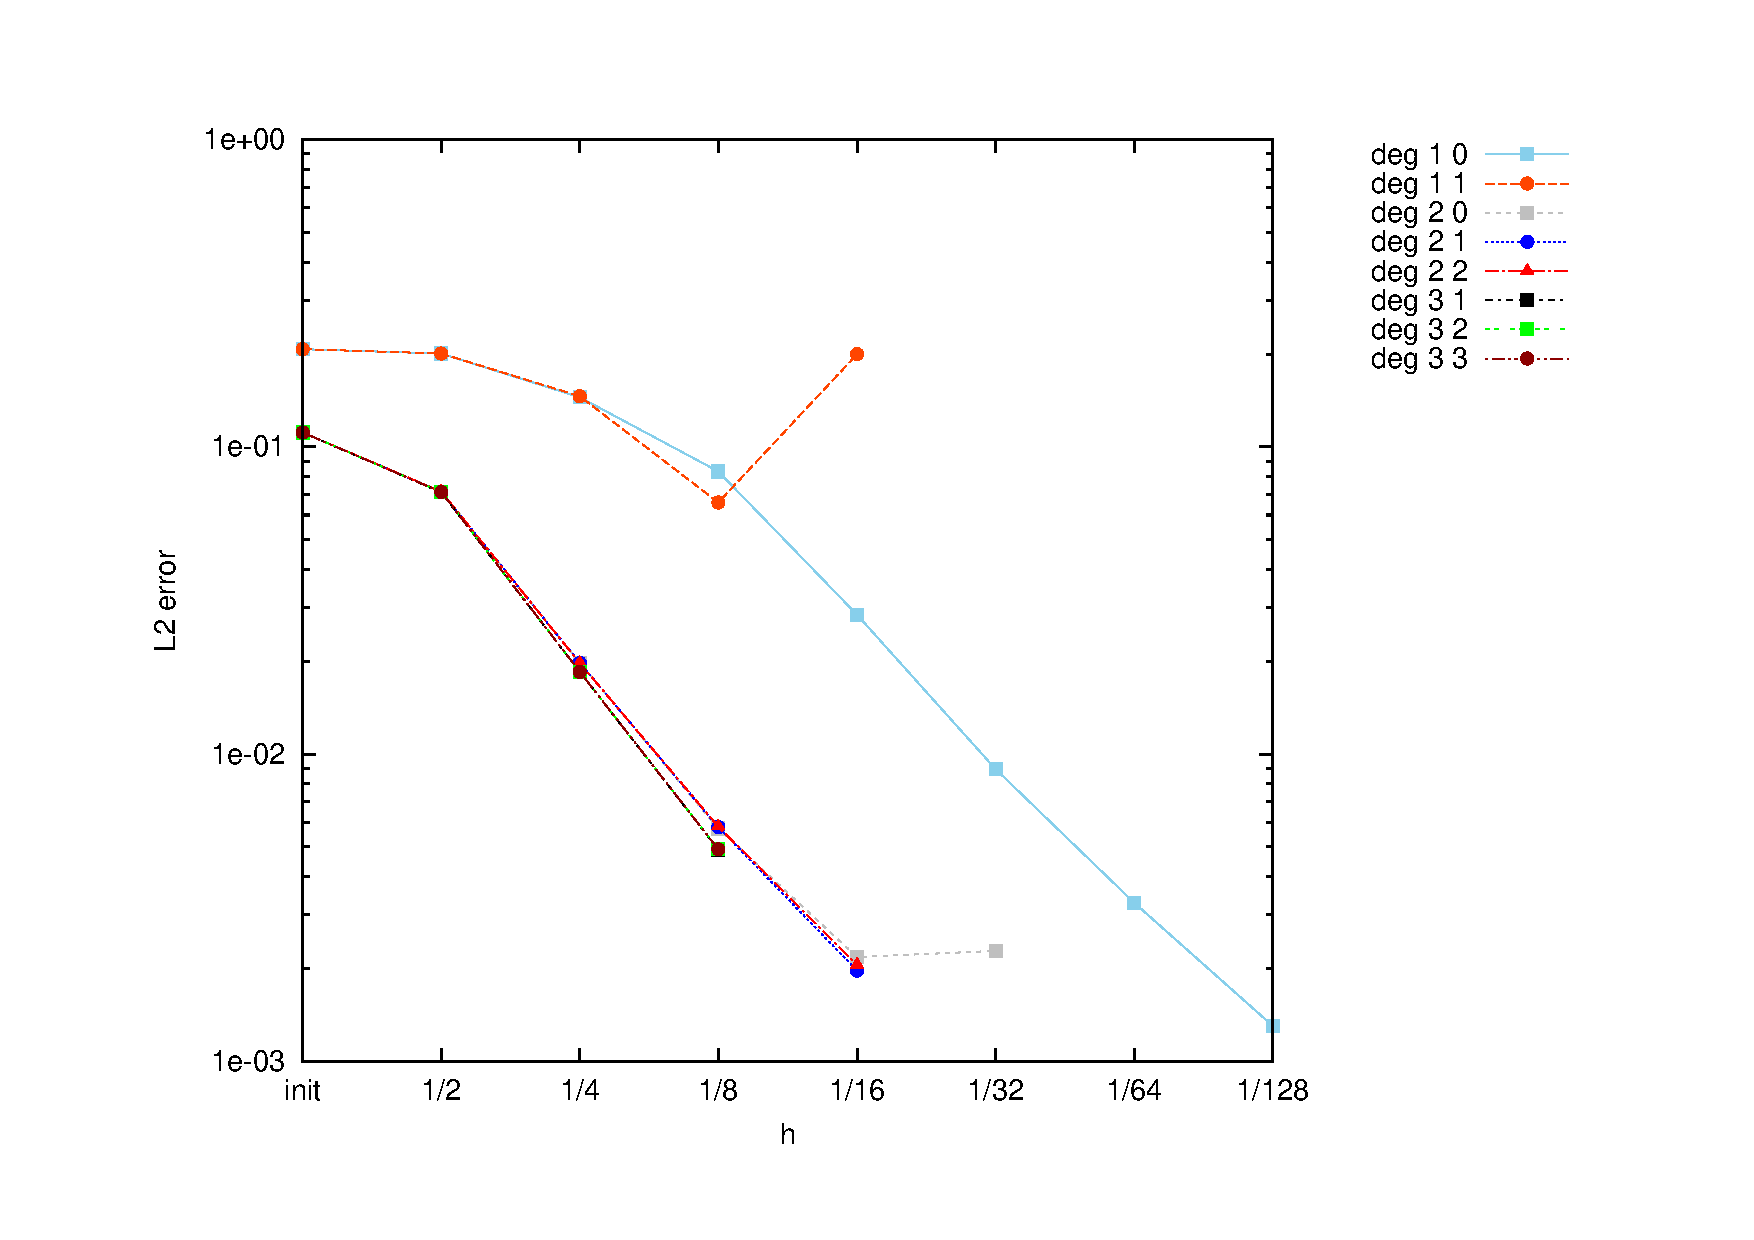
\includegraphics[scale =0.4]{plots/MA4_Neilan_GradJump_l2.pdf}
	\caption{$L^2$ errors for Test \ref{test dirac} and additional gradient jump penalty}
	\label{fig: l2 errors test 4 jump}
\end{figure}
	
\begin{figure}[H]
		\centering
		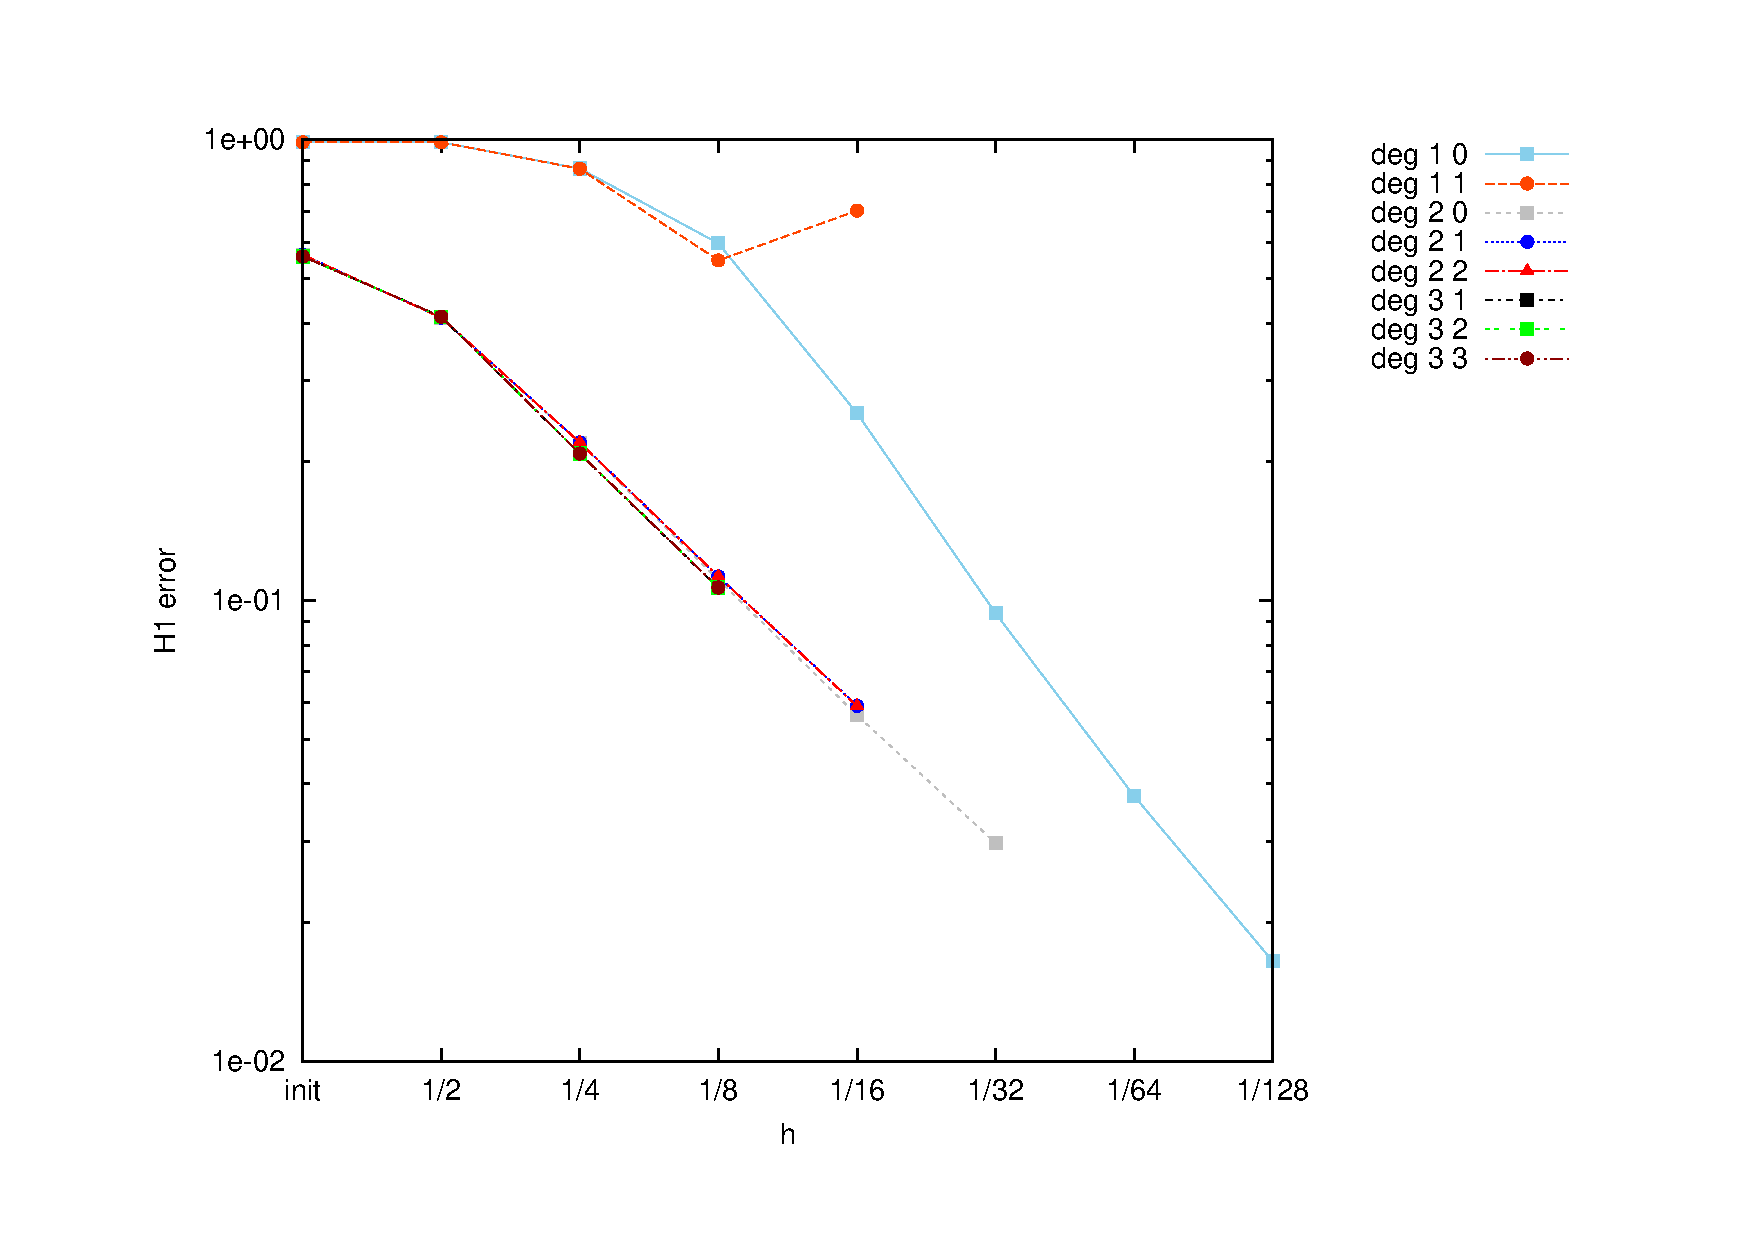
\includegraphics[scale =0.4]{plots/MA4_Neilan_GradJump_h1.pdf}
	\caption{$H^1$ errors for Test \ref{test dirac} and additional gradient jump penalty}
	\label{fig: h1 errors test 4 jump}
\end{figure}

\begin{table}[h]
	\centering
	\begin{subtable}[b]{0.45\textwidth}
		\centering
		\pgfplotstabletypeset[columns={iterations, l2error, h1error,N},
		every row 0 column 0/.style={set content=init},
		]{\MAFourJumpdegOneZero}
		\caption{Error for $k=1, k_{DH}=0$}
	\end{subtable}
	~
	\begin{subtable}[b]{0.45\textwidth}
		\centering
		\pgfplotstabletypeset[
		columns={iterations, l2error, h1error,N},
		every row 0 column 0/.style={set content=init},
		every row 5 column 1/.style={set content=-},
		every row 5 column 2/.style={set content=-},
		every row 5 column 3/.style={set content=-},
		every row 6 column 1/.style={set content=-},
		every row 6 column 2/.style={set content=-},
		every row 6 column 3/.style={set content=-},
		every row 7 column 1/.style={set content=-},
		every row 7 column 2/.style={set content=-},
		every row 7 column 3/.style={set content=-},
		]{\MAFourJumpdegTwoTwo}
		\caption{Error for $k=2, k_{DH}=2$}
	\end{subtable}
	\caption{Errors for Test \ref{test dirac} and additional gradient jump penalty}
	\label{tab: l2 errors test 4 jump}
\end{table}


\begin{table}[H]
\centering
\begin{subtable}[b]{0.45\textwidth}
	\centering
	\pgfplotstabletypeset
	{
		k $k_{DH}$ {numerical order}
		1 0 1.28471
		2 0 1.31145
		2 1 1.73123
		2 2 1.71168
	}
	\caption{Numerical order in $L^2$ norm}
	\end{subtable}
	\begin{subtable}[b]{0.45\textwidth}
	\centering
	\pgfplotstabletypeset
	{
		k $k_{DH}$ {numerical order}
		1 0 1.05121
		2 0 0.954061
		2 1 0.936276
		2 2 0.936544
	}
	\caption{Numerical order in $H^1$ norm}
	\end{subtable}
	\caption{Numerical order with jump penalty in Test \ref{test singularity}}
\label{tab: order jump 4}
\end{table}
